%---------------------------------------
\section{INTRODUCCIÓN} \label{sec:Introduccion}
%---------------------------------------
El presente documento pretender exponer las dificultades algebraicas que plantea el cálculo de la velocidad de avance generada a través del movimiento de onda viajera realizado por microorganismos \cite{Gray1955} y animales acuáticos (peces \textit{Carangiform}) \cite{Korkmaz2012,Korkmaz2011}. Exponer una solución a estas dificultades mediante computación numérica e interpretar y analizar los resultados ofrecidos por la solución propuesta.\\

El movimiento de onda viajera realizado por la mayoría de los peces, según la ictiología es doblando su cuerpo su cuerpo \cite{modeswim}. Este tipo de movimiento denominado \textit{``body and caudal fin''} (BCF) se encuentra categorizado en diferentes clases, de las cuáles el tipo \textit{Carangiform}  presenta la mayor similitud con el movimiento del flagelo de las células. El movimiento descrito por este tipo de peces fue sugerido originalmente por Lighthill \cite{FLM:368244}, y su expresión matemática es
\begin{eqnarray}
	\label{eq:fish_traveling_wave}
	y (x,t) = (c_1 x + c_2 x^2) \sin \left( \frac{2 \pi}{\lambda}  ( x - V_p t) \right),
\end{eqnarray}
donde $x$ es el desplazamiento sobre el eje principal, $V_p$ la velocidad de propagación de las ondas respecto al cuerpo y de sentido contrario a la velocidad de avance, $\lambda$ la longitud de onda y $c_1$ y $c_2$ los coeficientes lineal y cuadrático de la amplitud de la onda, respectivamente. Esta expresión recoge la dinámica del movimiento \textit{Carangiform} realizado desde el punto de unión del cuerpo hasta el extremo final de la cola \cite{Robotic_Fish,Robotic_Fish_speed,Robotic_Fish_3D}. Para recoger en una misma expresión la posibilidad de una onda viajera arm\'onica como la estudiada para los flagelos en \cite{gray1955propulsion}, se debe introducir un nuevo coeficiente $c_0$ quedando la expresión anterior de la forma
\begin{eqnarray}
	\label{eq:flag_fish_traveling_wave}
	y (x,t) = (c_0+c_1 x + c_2 x^2) \sin \left( \frac{2 \pi}{\lambda}  ( x - V_p t) \right).
\end{eqnarray}

En (\ref{eq:flag_fish_traveling_wave}), el coeficiente $c_0$ permite definir el movimiento armónico puro de la onda viajera, como se ilustra en la Figura~\ref{fig:FC}, pero no define el realizado por la cola de un pez. Es necesario sustituirlo por el coeficiente $c_1$, que impone la condición de contorno $y(0,t) = 0$, es decir, el inicio de la cola se encuentra unido a la cabeza en todo instante de tiempo. Sin embargo, dicho coeficiente define una onda viajera cuya amplitud crece linealmente en el eje principal (ver Figura~\ref{fig:FC}). Para corregir este comportamiento se introduce el término cuadrático $c_2$, con el cual es posible modular el crecimiento de la onda viajera para alcanzar una amplitud mantenida sobre el eje principal.

%\begin{figure}[t] %  figure placement: here, top, bottom, or page
 %  \vspace*{3mm}
%   \centering
  % 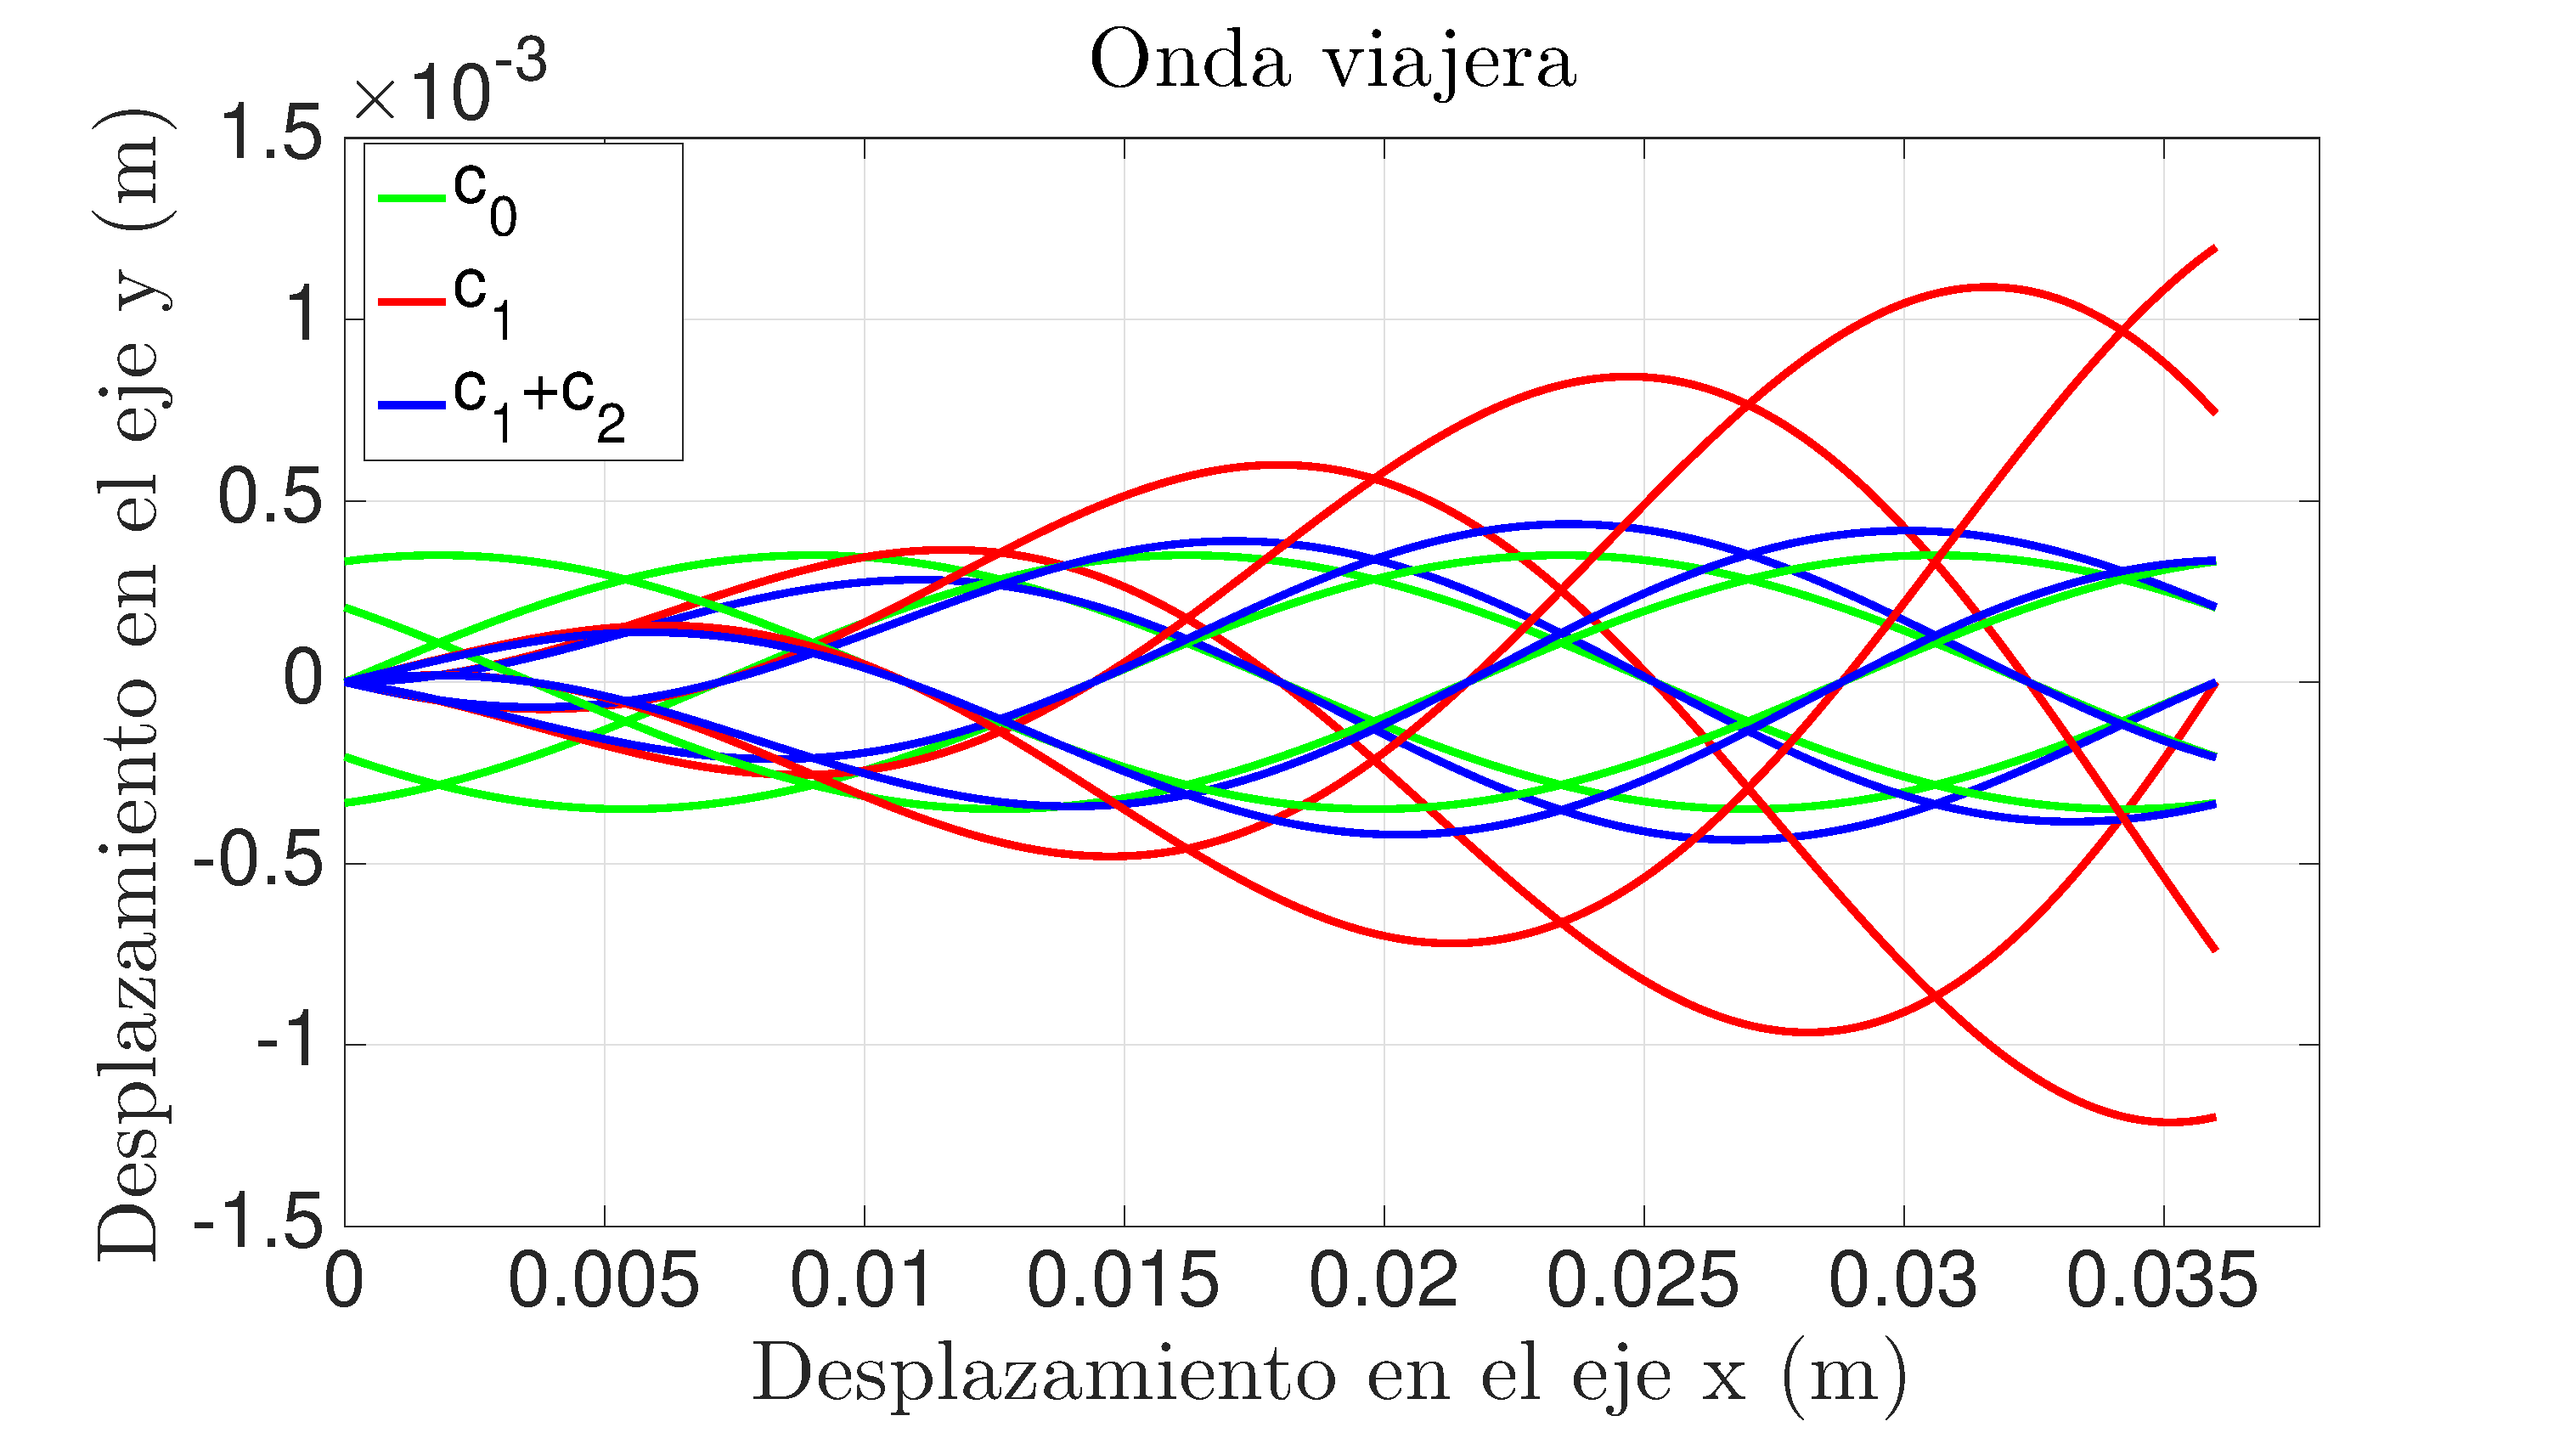
\includegraphics[width=0.5\textwidth]{Figuras/FC}
%  \caption{Comparación de la onda viajera para diferentes coeficientes de definición.}
 %  \label{fig:FC}
%\end{figure}  



% Foto del que describa el movimiento.